\documentclass{standalone}
\usepackage{tikz}
\usepackage{fontspec}
\usetikzlibrary{patterns}
\usetikzlibrary{arrows}

%: === TIPOGRAFÍA === (((
\setmainfont[
  BoldFont       = bodonibi,
	ItalicFont     = Century modern italic2.ttf,
	BoldItalicFont = bodonibi,
	SmallCapsFont  = lmromancaps10-regular.otf
]{Century_modern.ttf}
\DeclareSymbolFont{italics}{\encodingdefault}{\rmdefault}{m}{it}
\DeclareSymbolFontAlphabet{\mathit}{italics}
\ExplSyntaxOn
\int_step_inline:nnnn { `A } { 1 } { `Z }
 {  \exp_args:Nf \DeclareMathSymbol{\char_generate:nn{#1}{11}}{\mathalpha}{italics}{#1} }
\int_step_inline:nnnn { `a } { 1 } { `z } {  \exp_args:Nf \DeclareMathSymbol{\char_generate:nn{#1}{11}}{\mathalpha}{italics}{#1}}
\ExplSyntaxOff
% )))

\begin{document}

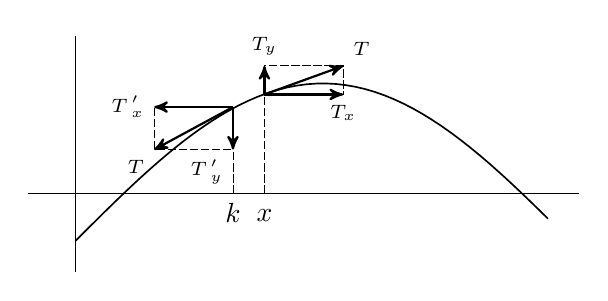
\begin{tikzpicture}[>=stealth', scale=2]
	\draw (-0.3,0) -- (3.2,0) (0,-0.5) -- (0,1);
	\draw [semithick , domain=0:3, samples = 50] plot(\x , {sin(\x r)-0.3});
	\draw [dash pattern = on 3pt off 1pt, very thin] (1,0) node [below] {\(k\)} --++ (0,0.55);
	\draw [dash pattern = on 3pt off 1pt, very thin] (1.2,0) node [below=0.8mm] {\(x\)} --++ (0,0.65);
	\draw [dash pattern = on 3pt off 1pt] (1.2,0.63) rectangle ++(0.5,{0.5*cos(1.2 r)});
	\draw [thick , ->] (1.2,0.63) --++ (0.5,{0.5*cos(1.2 r)}) node [above right] {\scriptsize \(T\)};
	\draw [thick , ->] (1.2,0.63) --++ (0,{0.5*cos(1.2 r)}) node [above] {\scriptsize \(T_y\)};
	\draw [thick , ->] (1.2,0.63) --++ (0.5,0) node [below] {\scriptsize \(T_x\)};
	\draw [thick , ->] (1,0.55) --++ (-0.5,{-0.5*cos(1 r)}) node [below left] {\scriptsize \(T\)};
	\draw [thick , ->] (1,0.55) --++ (0,{-0.5*cos(1 r)}) node [below left] {\scriptsize \(T\,'_y\)};
	\draw [thick , ->] (1,0.55) --++ (-0.5,0) node [left] {\scriptsize \(T\,'_x\)};
	\draw [dash pattern = on 3pt off 1pt] (1,0.55) rectangle ++(-0.5,{-0.5*cos(1 r)});
\end{tikzpicture}

\end{document}
